%% dk 20190521 prostate page 2

%\documentclass{article}

\documentclass[border=5]{standalone}

\usepackage{tikz}
%\usepackage{xcolor}
\usetikzlibrary{arrows,shapes,snakes,automata,backgrounds,petri, decorations.text,positioning, calc}

\begin{document}
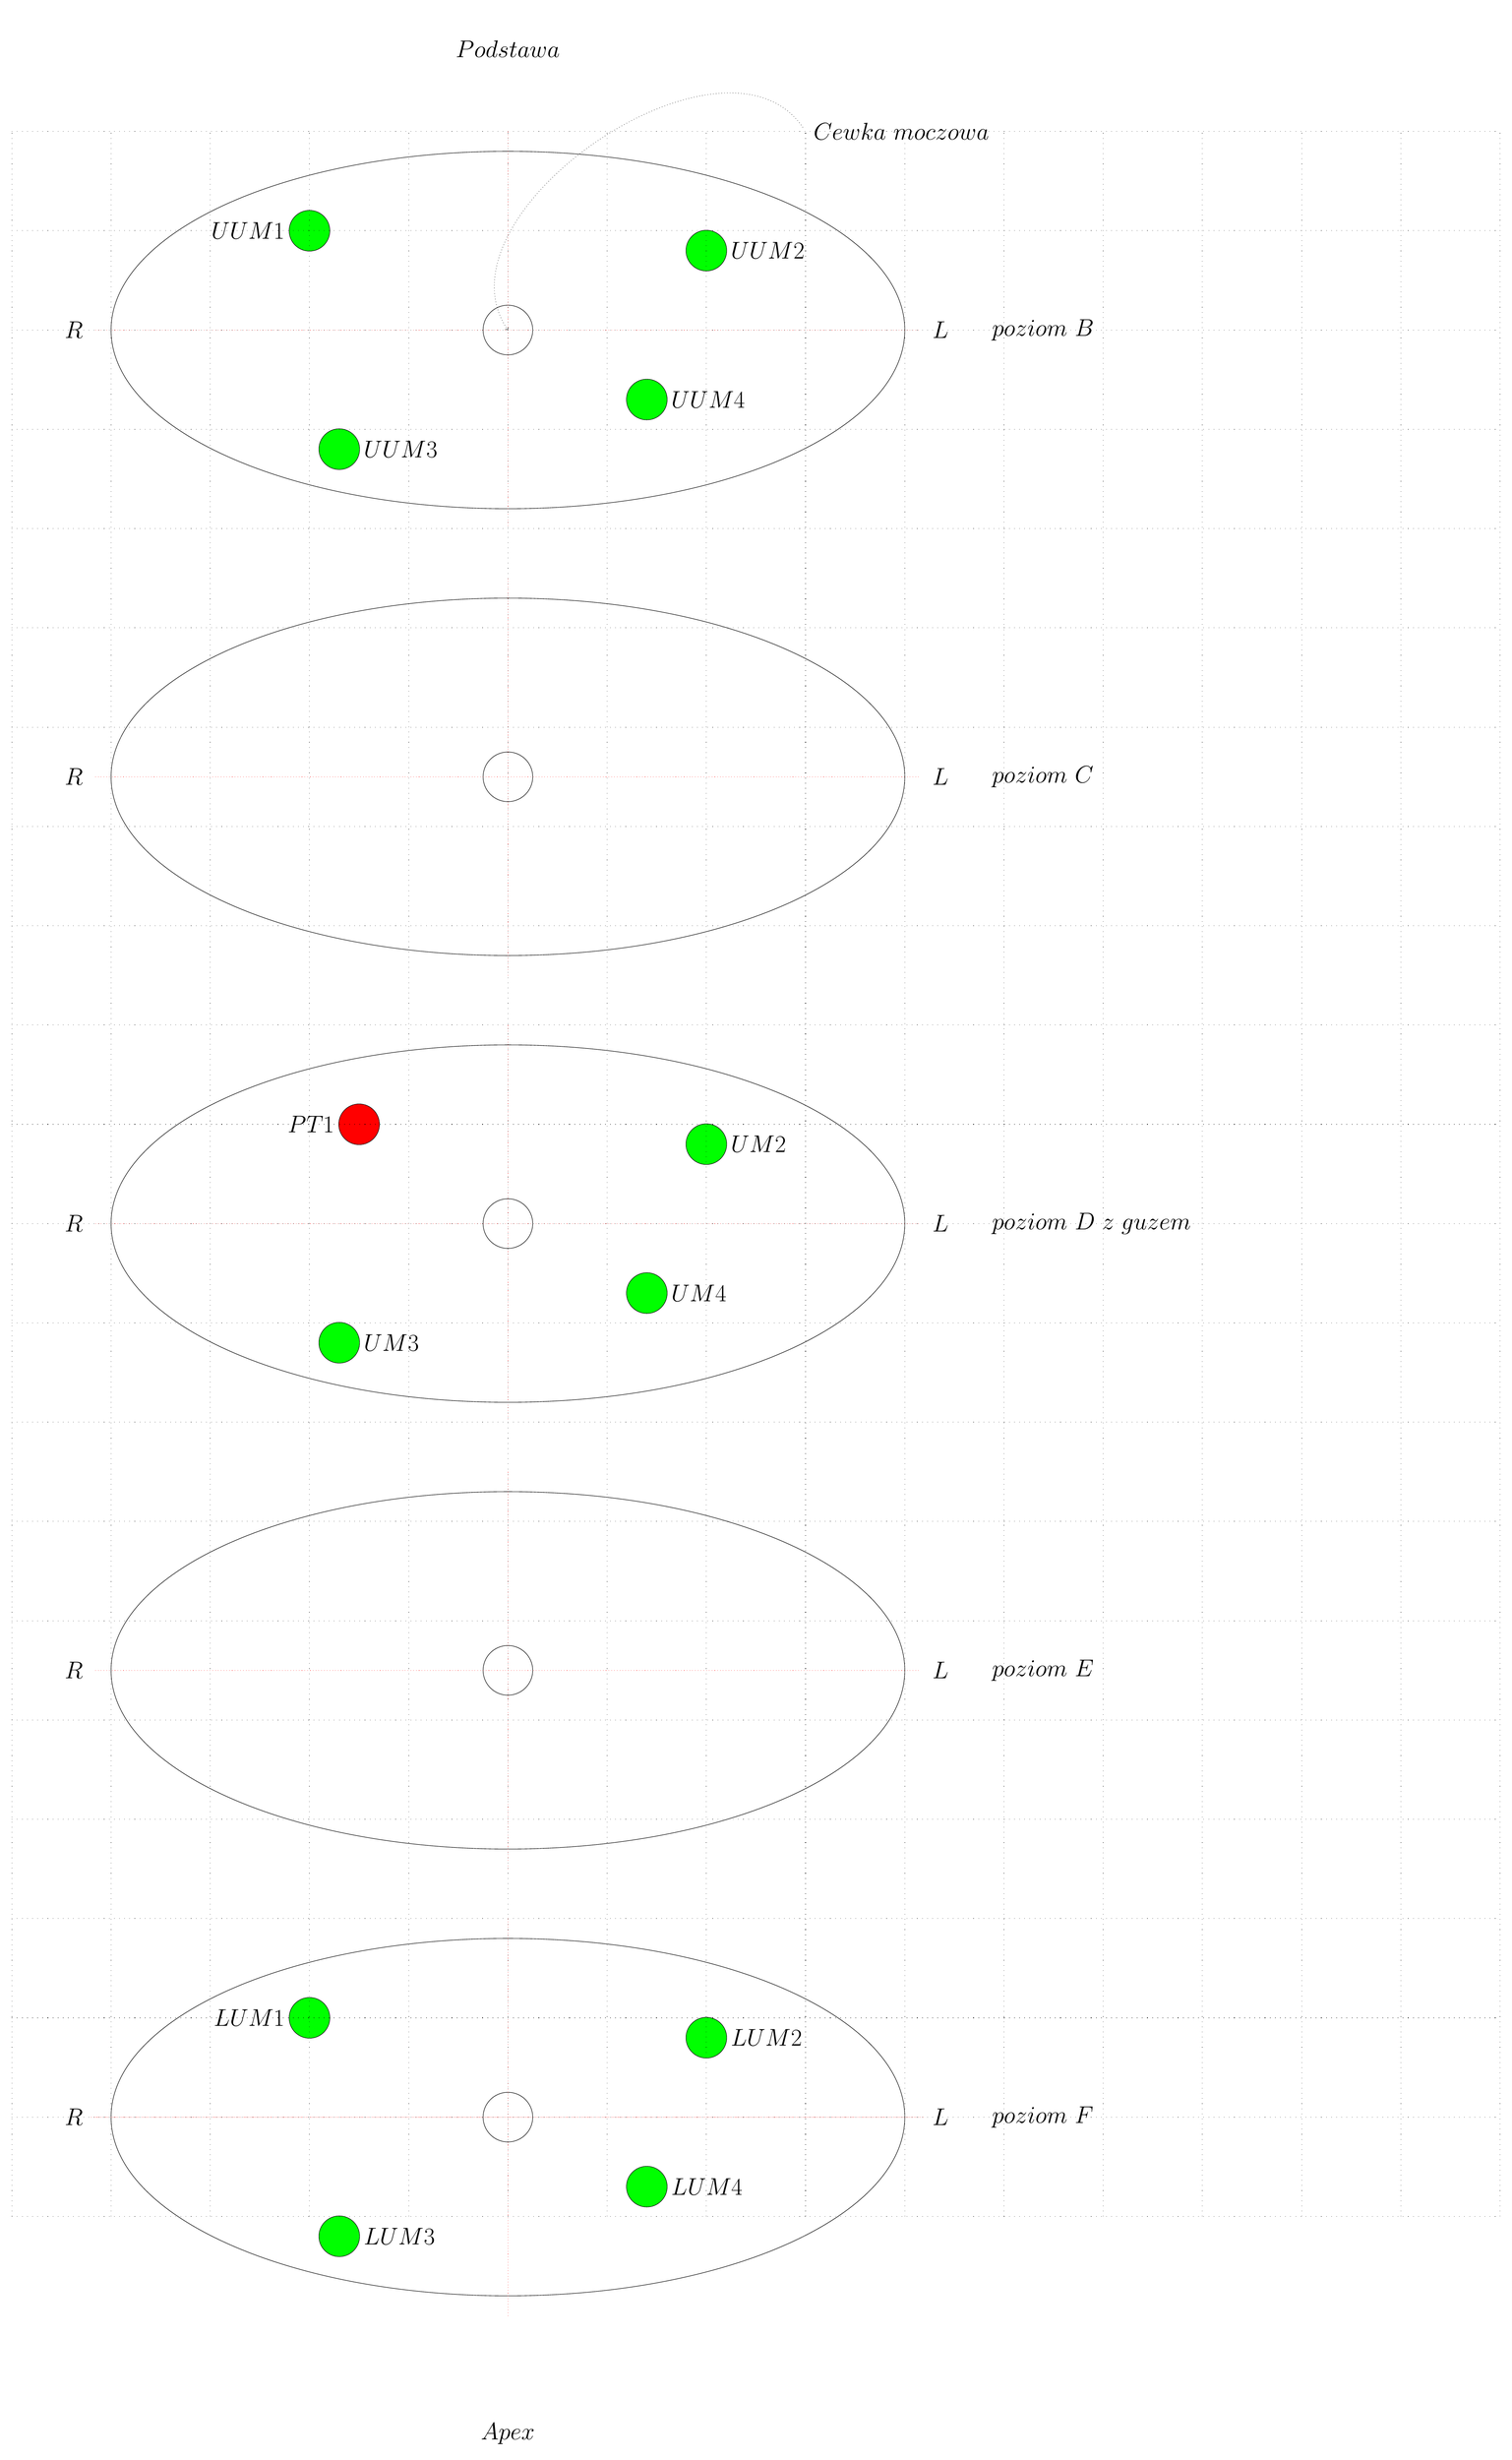
\begin{tikzpicture}[scale=3]

  %\draw [rounded corners=120mm,fill=gray!20] (0,10)--(10,10)--(5,1)--cycle;

  %\coordinate (EL1) at (0,14);
  %\foreach \i in {1,...,5}
  %{ }

  \def\x_el{4} % x ellipse
  \def\y_el{1.8} % x ellipse

  \coordinate (EL1) at (0,14);
  \coordinate (EL2) at ($(EL1) - (0,4.5)$);
  \coordinate (EL3) at ($(EL1) - 2*(0,4.5)$);
  \coordinate (EL4) at ($(EL1) - 3*(0,4.5)$);
  \coordinate (EL5) at ($(EL1) - 4*(0,4.5)$);



  \node [label=below:{\huge{$Podstawa$}} ] (Podstawa) at  ($(EL1) + (0,3)$) {};
  \node [label=right:{\huge{$Cewka\ moczowa$}} ] (cewka_label) at  ($(Podstawa) + (3,-1)$) {};


  \node [label=below:{\huge{$Apex$}} ] (Apex) at  ($(EL5) + (0,-3)$) {};



  \draw (EL1) ellipse (\x_el and \y_el);
  \draw (EL1) circle (0.25);
  \draw[dotted, ->]
  (cewka_label) [bend right=90]  to  (EL1);
  \node [label=left:{\huge{$R$}} ] (REL1) at  ($(EL1) + (-4.2,0)$) {};
  \node [label=right:{\huge{$L$}} ] (LEL1) at  ($(EL1) + (4.2,0)$) {};

  \node [label=right:{\huge{$ poziom\ B$}} ] (levELB) at  ($(LEL1) + (0.6,0)$) {};

  \draw[dotted, red] (REL1) --  (LEL1);
  \draw[dotted, red] ($(EL1) + (0,-2)$) --  ($(EL1) + (0,2)$);

  \draw (EL2) ellipse (\x_el and \y_el);
  \draw (EL2) circle (0.25);
  \node [label=left:{\huge{$R$}} ] (REL2) at  ($(EL2) + (-4.2,0)$) {};
  \node [label=right:{\huge{$L$}} ] (LEL2) at  ($(EL2) + (4.2,0)$) {};
  \node [label=right:{\huge{$ poziom\ C$}} ] (levELC) at  ($(LEL2) + (0.6,0)$) {};

  \draw[dotted, red] (REL2) --  (LEL2);


  \draw[dotted, red] ($(EL2) + (0,-2)$) --  ($(EL2) + (0,2)$);

  \draw (EL3) ellipse (\x_el and \y_el);
  \draw (EL3) circle (0.25);
  \node [label=left:{\huge{$R$}} ] (REL3) at  ($(EL3) + (-4.2,0)$) {};
  \node [label=right:{\huge{$L$}} ] (LEL3) at  ($(EL3) + (4.2,0)$) {};
  %\node (levELD)  at  ($(LEL3) + (0.6,0)$) [align=left] {\huge poziom\ D\\z\ guzem}   ;

  \node [label=right:{\huge{$ poziom\ D\ z\ guzem$}} ] (levELD) at  ($(LEL3) + (0.6,0)$) {};


  \draw[dotted, red] (REL3) --  (LEL3);

  \draw[dotted, red] ($(EL3) + (0,-2)$) --  ($(EL3) + (0,2)$);

  \draw (EL4) ellipse (\x_el and \y_el);
  \draw (EL4) circle (0.25);
  \node [label=left:{\huge{$R$}} ] (REL4) at  ($(EL4) + (-4.2,0)$) {};
  \node [label=right:{\huge{$L$}} ] (LEL4) at  ($(EL4) + (4.2,0)$) {};
  \node [label=right:{\huge{$ poziom\ E$}} ] (levELE) at  ($(LEL4) + (0.6,0)$) {};

  \draw[dotted, red] (REL4) --  (LEL4);

  %\draw[dotted, red] ($(EL4) + (-4.2,0)$) --  ($(EL4) + (4.2,0)$);
  \draw[dotted, red] ($(EL4) + (0,-2)$) --  ($(EL4) + (0,2)$);

  \draw (EL5) ellipse(\x_el and \y_el);
  \draw (EL5) circle (0.25);
  \node [label=left:{\huge{$R$}} ] (REL5) at  ($(EL5) + (-4.2,0)$) {};
  \node [label=right:{\huge{$L$}} ] (LEL5) at  ($(EL5) + (4.2,0)$) {};
  \node [label=right:{\huge{$ poziom\ F$}} ] (levELF) at  ($(LEL5) + (0.6,0)$) {};

  \draw[dotted, red] (REL5) --  (LEL5);

  \draw[dotted, red] ($(EL5) + (-4.2,0)$) --  ($(EL5) + (4.2,0)$);
  \draw[dotted, red] ($(EL5) + (0,-2)$) --  ($(EL5) + (0,2)$);

  %%% samples
  %% level B
  \node (UUM1) at ($(EL1) + (-2,1.0) $) [circle,draw=black,fill=green,inner sep=0pt,minimum size=35pt,label=left:{\huge{$UUM1$}}]  {};

  \node (UUM2) at ($(EL1) + (2,0.8) $) [circle,draw=black,fill=green,inner sep=0pt,minimum size=35pt,label=right:{\huge{$UUM2$}}]  {};

  \node (UUM3) at ($(EL1) + (-1.7,-1.2) $) [circle,draw=black,fill=green,inner sep=0pt,minimum size=35pt,label=right:{\huge{$UUM3$}}]  {};

  \node (UUM4) at ($(EL1) + (1.4,-0.7) $) [circle,draw=black,fill=green,inner sep=0pt,minimum size=35pt,label=right:{\huge{$UUM4$}}]  {};

  %% level tumor
  \node (PT1) at ($(EL3) + (-1.5,1.0) $) [circle,draw=black,fill=red,inner sep=0pt,minimum size=35pt,label=left:{\huge{$PT1$}}]  {};

  \node (UM2) at ($(EL3) + (2,0.8) $) [circle,draw=black,fill=green,inner sep=0pt,minimum size=35pt,label=right:{\huge{$UM2$}}]  {};

  \node (UM3) at ($(EL3) + (-1.7,-1.2) $) [circle,draw=black,fill=green,inner sep=0pt,minimum size=35pt,label=right:{\huge{$UM3$}}]  {};

  \node (UM4) at ($(EL3) + (1.4,-0.7) $) [circle,draw=black,fill=green,inner sep=0pt,minimum size=35pt,label=right:{\huge{$UM4$}}]  {};

  %% level 5
  \node (LUM1) at ($(EL5) + (-2,1.0) $) [circle,draw=black,fill=green,inner sep=0pt,minimum size=35pt,label=left:{\huge{$LUM1$}}]  {};

  \node (LUM2) at ($(EL5) + (2,0.8) $) [circle,draw=black,fill=green,inner sep=0pt,minimum size=35pt,label=right:{\huge{$LUM2$}}]  {};

  \node (LUM3) at ($(EL5) + (-1.7,-1.2) $) [circle,draw=black,fill=green,inner sep=0pt,minimum size=35pt,label=right:{\huge{$LUM3$}}]  {};

  \node (LUM4) at ($(EL5) + (1.4,-0.7) $) [circle,draw=black,fill=green,inner sep=0pt,minimum size=35pt,label=right:{\huge{$LUM4$}}]  {};



  \draw[loosely  dotted] (-5,-5) grid (10,16);
\end{tikzpicture}
\end{document}